\section{Physical four-mode transport theory}
\subsection{Symmetry and the fixed mode hierarchy}
The hierarchy first retains the active current response, then an independent active valley displacement, then passive current and finally passive valley polarization. These coordinates distinguish carrying current from changing the partner populations. We construct a physical real basis from the DC reference and hold it fixed in frequency. Let $p_r=\sqrt w\,s\,1_r$ denote the weighted partner-population displacement in sector $r$, implicitly projected into the orthonormal time-reversal-odd coordinates. Starting from
\begin{gather}
U_{\rm raw}=(g_{A0},p_A,b_P,p_P),\nonumber\\
U=U_{\rm raw}\mathsf T,\quad U^TU=I.\label{eq:basis}
\end{gather}
we orthonormalize in this order. Sector-supported vectors are embedded with zeros in the other sector. Thus $u_1=g_{A0}/G$, $G=\norm{g_{A0}}$, and $u_2$ is the normalized component of $p_A$ orthogonal to $u_1$. The passive columns are normalized current and partner population. Their overlap vanishes for the untilted passive contour used here. The saved matrix $\mathsf T$ specifies every normalization and subtraction.

The first column is the full uncoupled current response, not generally $v_x$ times a lifetime. It retains the active sector's own non-scalar relaxation. The second column therefore describes an independent active valley distortion; after orthogonalization it need not be a pure population or have zero current overlap. The passive current has zero partner-population difference, while the fourth column changes the populations with opposite signs. Neither is a total active-to-passive charge-transfer mode, which is even under time reversal and absent from the driven space.

For the Hamiltonian of Sec.~IV, time reversal sends $(s,q_x,q_y)$ to $(-s,-q_x,-q_y)$. The remaining physical mirror sends it to $(-s,-q_x,q_y)$ with internal action $\sigma_x$. All four displacements are odd under both operations and even under their combined local $q_y$ reflection. Simple partner exchange at equal local angle is not a symmetry of the tilted active contours; assigning its parity to the active columns would be incorrect. Figure~\ref{fig:model} summarizes the physical content.

Models M1--M4 retain the first one through four columns, without changing their order or fitting additional harmonics. For $U_m=(u_1,\ldots,u_m)$,
\begin{align}
K_m&=U_m^TLU_m,\quad d_m=U_m^Tb,\quad j_m=U_m^Th,\nonumber\\
(K_m+i\omega I)x_m&=d_m,\quad g_m=U_mx_m,\quad H_m=j_m^Tx_m.
\end{align}
Every projection uses the same full collision operator. In particular, M1 and M2 retain intersector scattering-out even though passive displacement is frozen; they are not the active-only omission reference. Incremental differences $H_m-H_{m-1}$ describe this ordered ablation, not independent scattering-channel contributions.

We also evaluate $\sigma_{xx,m}=b^Tg_m$, $\chi_m=-H_m/2$ and
\begin{equation}
Q=\frac{H W}{\sigma_{xx}D},\qquad
Q_A=\frac{H W_A}{\sigma_A D},\label{eq:Q}
\end{equation}
where $D=h^Tb$, $W=b^Tb$, $W_A=b_A^Tb_A$ and $\sigma_A=b_A^Tg_A$. These ratios compare Hall readout with current relaxation. Projection errors use the full observable as denominator, distinct from the omission error in Eq.~\eqref{eq:error}. Distribution error is $\norm{g_m-g}/\norm g$ in weighted coordinates. The $x$-driven basis is not used to approximate the different symmetry sector driven by $v_y$.

\begin{figure*}[!tp]\centering
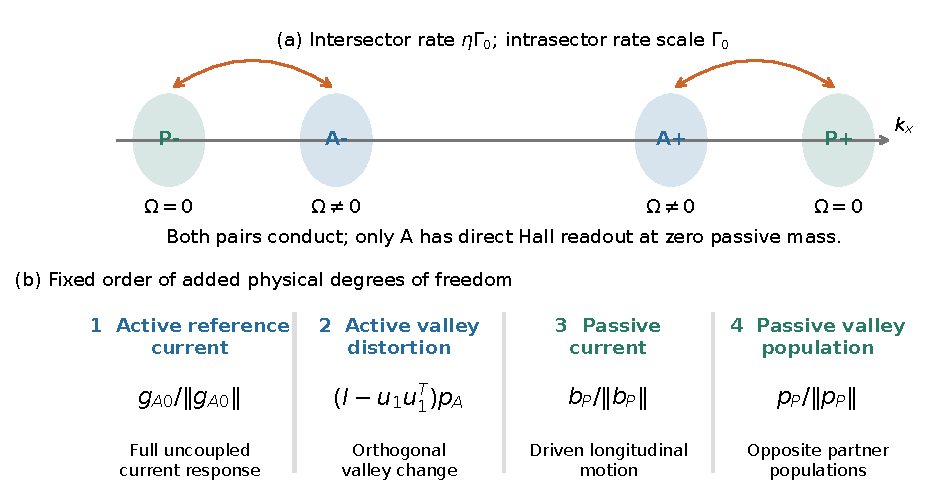
\includegraphics[width=\textwidth]{../figures/main/figure_1_physical_modes.pdf}
\caption{Model and physical coordinates. (a) Hall-active and Hall-silent conducting pairs with intra- and intersector scattering; the contours are schematic. (b) The fixed sequence of physical degrees of freedom. The active distortion is normalized after removing its reference-current component. The passive modes have zero direct Hall weight at $m_P=0$, but can transmit drive and relaxation changes to the active pair. All columns use the contour-weighted inner product.}\label{fig:model}
\end{figure*}

\subsection{Contact closure and finite-range leakage}
For contact disorder, $|u_i^\dagger u_j|^2=(1+\bm n_i\cdot\bm n_j)/2$. Time reversal cancels each sector's integrated Bloch vector, so scattering out has the constant rate $\Gamma_0(D_r+\eta D_{\bar r})/2$, where $D_r$ is its density of states. The constant incoming moment vanishes for an odd displacement. On a contour $\delta=\mu-E=stq_x+d$,
\begin{align}
n_y&=(v_x-st)/v,\\
n_z&=\frac m\delta\left[s(1-t^2/v^2)+(t/v^2)v_x\right].\label{eq:closure}
\end{align}
The remaining component $n_x=-vq_y/d$ is odd under local $q_y$ reflection and does not enter this drive sector. Incoming moments therefore close on the two functions $v_x,s$ in each sector. This space contains the drive and is invariant under $L$. Replacing active velocity by its uncoupled response leaves the same span. At $m_P=t_P=0$, the passive population has zero drive and decouples, so M3 already solves the contact problem exactly. Finite range makes the outgoing rate angle dependent and prevents the incoming kernel from factoring into this finite set of moments.

With $P_U=UU^T$, define
\begin{align}
R_{\rm inv}&=(I-P_U)LU,\\
\rho_{\rm abs}&=\norm{R_{\rm inv}}_2,&
\rho_{\rm rel}&=\frac{\norm{R_{\rm inv}}_2}{\norm{LU}_2}.\label{eq:leak}
\end{align}
Both are spectral norms; separate Frobenius diagnostics are supplied. Closure is a property of the operator and basis, not a synonym for an accurate observable.

The drive can also miss the finite-range space. For $b_\perp=(I-P_U)b$, the reduced residual and exact response error obey
\begin{align}
r_b&=b-(L+i\omega I)Ux_4=b_\perp-R_{\rm inv}x_4,\\
H-H_4&=h^T(L+i\omega I)^{-1}r_b=z^Tr_b.\label{eq:projectionerror}
\end{align}
Here $(L+i\omega I)^Tz=h$ and $U^Tr_b=0$. Consequently $z$ may be replaced by $(I-P_U)z$. At DC a rigorous estimate is
\begin{equation}
|H-H_4|\leq\norm{(I-P_U)z}\norm{r_b}
\leq\frac{\norm{r_h}\norm{r_b}}{\lambda_{\min}(L)},\label{eq:dualbound}
\end{equation}
where $r_h=h-LU K_4^{-1}U^Th$ is the Galerkin dual residual; the second inequality follows by subtracting the reduced dual solution before projection. In turn $\norm{r_b}\leq\norm{b_\perp}+\rho_{\rm abs}\norm{x_4}$. Thus leakage alone cannot bound Hall error without drive, relaxation and readout information. These standard residual estimates explain the diagnostics; no computational advantage is inferred from an exact dual solve.

\subsection{Scalar and Hall-sensitive redistribution}
At DC the active reference defines the exact decomposition
\begin{align}
\alpha_*&=\frac{g_{A0}^\dagger g_A}{g_{A0}^\dagger g_{A0}},\qquad r_A=g_A-\alpha_*g_{A0},\nonumber\\
H-H_0&=S+T,\quad S=(\alpha_*-1)H_0,\quad T=h_A^Tr_A.\label{eq:ST}
\end{align}
The terms $S$ and $T$ are projection-defined diagnostic components, not independently measurable microscopic currents. Their separation depends on the stated contour norm and active reference. In M4, $S_4=j_1(x_1-G)$ and $T_4=j_2x_2$: the active valley distortion is the retained shape coordinate. Eliminating the two passive coordinates gives
\begin{equation}
\begin{pmatrix}a&c\\c&d\end{pmatrix}\binom{x_1}{x_2}
=\binom{p_1}{p_2}.\label{eq:shapeamp}
\end{equation}
Then $x_2=(p_2-cp_1/a)/\kappa$ with $\kappa=d-c^2/a$. Passive feedback changes the effective rates, and transmitted passive drive changes both entries of $p$. The shape response is a residual forcing divided by a positive Schur stiffness and multiplied by its Hall overlap. The stiffness is not itself a collision eigenvalue. This representation predicts scalar or shape dominance from amplitudes and readout, while allowing their signed contributions to oppose.
